\documentclass{article}

\input{physicsPream}

\usepackage{listings}
\lstset
{
  language=Matlab,
  numbers=left
}


\begin{document}

%----------BEGIN TITLEPAGE----------

\begin{titlepage}

  \title{PDE Project: Problem 7.2.4}
  \date{December 6, 2018}
  \author{Timothy Fraizer\\
          Lani Oramas\\
          Jason Williams\\
          Ryan Wojtyla\\}

  \maketitle

  \thispagestyle{empty}

\end{titlepage}

%-----------END TITLEPAGE-----------

%----------BEGIN PART A----------

\section*{Part A}

\qq Part A of the problem asks us to plot \(y_n = e^{\frac{x^2}{2}} H_n(x)\)
when \(n = [0,1,2,3]\), where \(H_n(x)\) is the Hermite polynomial. The plot,
Figure \ref{gph:hermite}, was generated with the code displayed in Figure
\ref{cod:hermite}.

\begin{figure}[H]
  \begin{center}
    \lstinputlisting{../MATLAB/hermite.m}
  \end{center}
  \caption{The MATLAB code for generating the plots of \(y_n = e^{\frac{x^2}{2}}
    H_n(x)\) for \(n = [0,1,2,3]\).}
  \label{cod:hermite}
\end{figure}

\begin{figure}[H]
  \begin{center}
    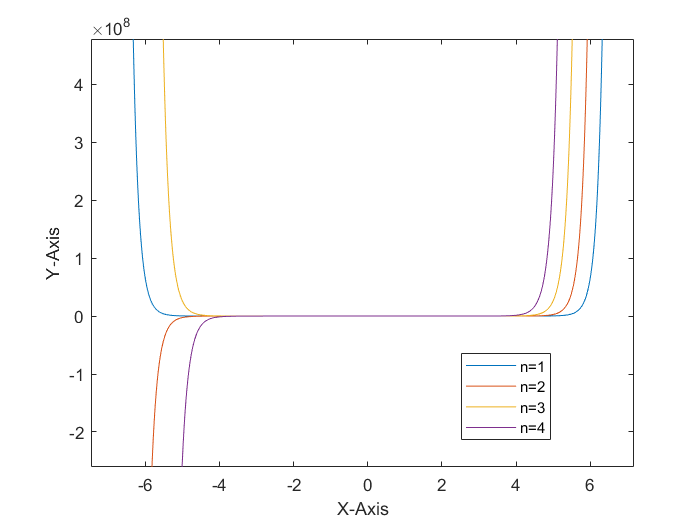
\includegraphics[scale=0.7]{MATLAB2.png}
  \end{center}
  \caption{The plots of \(y_n = e^{\frac{x^2}{2}}H_n(x)\) for \(n = [0,1,2,3]\).}
  \label{gph:hermite}
\end{figure}

%-----------END PART A-----------

%----------BEGIN PART B----------

\section*{Part B}

\qq Part B asks us to use the MATLAB function {\tt bvp4c} to find the first four
eigenfunctions of the second order differential equation
\(y\prime\prime + (\lambda - x^2) y = 0\) in the range \(-L \leq x \leq L\) with
the boundary conditions \(y(-L) = y(L) = 0\). Unfortunately, we had some trouble
implementing {\tt bvp4c} in code, Figure \ref{cod:partB}. We could not come up
with a valid initial guess of the solution, the function on line 27. MATLAB
complained that a singular Jacobian was encountered, which indicates that the
solution diverges. We do not know how to guess a solution that does not produce
that error, i.e. one that does not diverge.

\begin{figure}[H]
  \begin{center}
    \lstinputlisting{../MATLAB/mat4bvp.m}
  \end{center}
  \caption{The attempted code for finding the eigenfunctions of Part B.}
  \label{cod:partB}
\end{figure}

%-----------END PART B-----------

\end{document}
